\documentclass[9.2pt,twocolumn]{article}
\usepackage{lmodern}
\usepackage{amssymb,amsmath}
\usepackage{ifxetex,ifluatex}
\usepackage{fixltx2e} % provides \textsubscript
\ifnum 0\ifxetex 1\fi\ifluatex 1\fi=0 % if pdftex
  \usepackage[T1]{fontenc}
  \usepackage[utf8]{inputenc}
\else % if luatex or xelatex
  \ifxetex
    \usepackage{mathspec}
  \else
    \usepackage{fontspec}
  \fi
  \defaultfontfeatures{Ligatures=TeX,Scale=MatchLowercase}
\fi
% use upquote if available, for straight quotes in verbatim environments
\IfFileExists{upquote.sty}{\usepackage{upquote}}{}
% use microtype if available
\IfFileExists{microtype.sty}{%
\usepackage{microtype}
\UseMicrotypeSet[protrusion]{basicmath} % disable protrusion for tt fonts
}{}
\usepackage[left=1.5cm,right=1.5cm,top=2.2cm,bottom=2.2cm]{geometry}
\usepackage{hyperref}
\PassOptionsToPackage{usenames,dvipsnames}{color} % color is loaded by hyperref
\hypersetup{unicode=true,
            pdftitle={Ethiopia},
            pdfauthor={Commitment to Human Capital - Scorecard},
            colorlinks=true,
            linkcolor=Maroon,
            citecolor=Blue,
            urlcolor=blue,
            breaklinks=true}
\urlstyle{same}  % don't use monospace font for urls
\usepackage{graphicx,grffile}
\makeatletter
\def\maxwidth{\ifdim\Gin@nat@width>\linewidth\linewidth\else\Gin@nat@width\fi}
\def\maxheight{\ifdim\Gin@nat@height>\textheight\textheight\else\Gin@nat@height\fi}
\makeatother
% Scale images if necessary, so that they will not overflow the page
% margins by default, and it is still possible to overwrite the defaults
% using explicit options in \includegraphics[width, height, ...]{}
\setkeys{Gin}{width=\maxwidth,height=\maxheight,keepaspectratio}
\IfFileExists{parskip.sty}{%
\usepackage{parskip}
}{% else
\setlength{\parindent}{0pt}
\setlength{\parskip}{6pt plus 2pt minus 1pt}
}
\setlength{\emergencystretch}{3em}  % prevent overfull lines
\providecommand{\tightlist}{%
  \setlength{\itemsep}{0pt}\setlength{\parskip}{0pt}}
\setcounter{secnumdepth}{0}
% Redefines (sub)paragraphs to behave more like sections
\ifx\paragraph\undefined\else
\let\oldparagraph\paragraph
\renewcommand{\paragraph}[1]{\oldparagraph{#1}\mbox{}}
\fi
\ifx\subparagraph\undefined\else
\let\oldsubparagraph\subparagraph
\renewcommand{\subparagraph}[1]{\oldsubparagraph{#1}\mbox{}}
\fi

%%% Use protect on footnotes to avoid problems with footnotes in titles
\let\rmarkdownfootnote\footnote%
\def\footnote{\protect\rmarkdownfootnote}

%%% Change title format to be more compact
\usepackage{titling}

% Create subtitle command for use in maketitle
\providecommand{\subtitle}[1]{
  \posttitle{
    \begin{center}\large#1\end{center}
    }
}

\setlength{\droptitle}{-2em}

  \title{Ethiopia}
    \pretitle{\vspace{\droptitle}\centering\huge}
  \posttitle{\par}
    \author{Commitment to Human Capital - Scorecard}
    \preauthor{\centering\large\emph}
  \postauthor{\par}
    \date{}
    \predate{}\postdate{}
  
\usepackage{fancyhdr}

\pagestyle{fancy}

\usepackage[table]{xcolor} \usepackage{xcolor} \usepackage{graphicx} \usepackage{eurosym} \usepackage{booktabs,xcolor}

\rhead{Africa Human Capital Project - \today}
\rfoot[C]{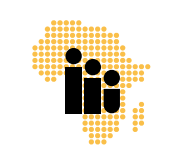
\includegraphics[width=2cm]{static/footer3.png}}
\fancypagestyle{plain}{\pagestyle{fancy}} \pagenumbering{gobble}

\usepackage{pagecolor}

\pagecolor{white}

\usepackage{fourier} \usepackage[fontsize=8.7pt]{scrextend} \usepackage{float} \usepackage[utf8]{inputenc}

\begin{document}
\maketitle

\definecolor{bondiblue}{rgb}{0.0, 0.58, 0.71}
\newcommand\boldblue[1]{\textcolor{bondiblue}{\textbf{#1}}}

This note presents a snapshot of the country's commitment on the human
capital agenda and the main actions being taken by the World Bank Group
to support the government.

\hypertarget{section}{%
\subsubsection{\texorpdfstring{\textcolor{bondiblue}{\textbf{H\small{UMAN CAPITAL CONTEXT}}}}{}}\label{section}}

\begin{itemize}
\item
  In Ethiopia the productivity as a future worker of a child born today
  is \textbf{38 percent} as much as it could be. The HCI has three
  components: survival to age 5, health, and education. For more
  information on human capital outcomes and the HCI, please see the
  country two-pager on
  \textcolor{bondiblue}{\textbf{www.worldbank.org/humancapitalproject}}
\item
  \textbf{Social Protection Coverage} In Ethiopia\textbf{13 percent} of
  the population is covered by social safety net programs. This is lower
  than both the average for its region (23) and the average for its
  income group (17).
\item
  \textbf{Open Defecation.} In Ethiopia, data on the percentage of the
  population that practices open defecation do not exist. The average
  for the country's region is 25 percent and for its income group is 25
  percent.
\end{itemize}

\hypertarget{section-1}{%
\subsubsection{\texorpdfstring{\textcolor{bondiblue}{\textbf{W\small{OMEN'S EMPOWERMENT}}}}{}}\label{section-1}}

\begin{itemize}
\item
  \textbf{Total Fertility Rate.} In Ethiopia, the total fertility rate
  is \textbf{4}. This is lower than both the average for its region (4)
  and the average for its income group (5).
\item
  \textbf{Adolescent Fertility Rate.} In Ethiopia, there are \textbf{62
  births} per 1,000 women ages 15-19. This is lower than both the
  average for its region (95)and the average for its income group (94).
\item
  \textbf{Contraceptive Prevalence.} In Ethiopia, \textbf{37 percent} of
  women ages 15-49 uses some form of contraceptive method. This is
  higher than both the average for its region (31) and the average for
  its income group (28).
\item
  \textbf{Women, Business and the Law Index.} This index measures gender
  inequality in the law and identifies barriers to women's economic
  participation, and a larger value shows higher gender equity.In
  Ethiopia, the value is \textbf{72} out of 100. This is higher than
  both the average for its region (70) and the average for its income
  group (68).
\item
  \textbf{Net Enrolment Rate in Secondary School.} In Ethiopia,
  \textbf{30 percent} of women of secondary-school age are enroled in
  school. This is lower than the average for its region (35) but higher
  than the average for its income group (29).
\end{itemize}

\hypertarget{section-2}{%
\subsubsection{\texorpdfstring{\textcolor{bondiblue}{\textbf{W\small{HOW IS THE COUNTRY DOING?}}}}{}}\label{section-2}}

Ethiopia is part of a network of countries committed to the Human
Capital agenda.

\begin{itemize}
\item
  \textbf{Health Spending.} Ethiopia spends \textbf{6 percent} of its
  government budget on health. This is lower than both the regional
  average (7.6) and the average for its income group (6.8).
\item
  \textbf{Education Spending.} Ethiopia spends \textbf{27.1 percent} of
  its government budget on education. This is higher than both the
  regional average (15.3) and the average for its income group (15.5).
\item
  \textbf{Social Protection Spending.} Ethiopia spends \textbf{10.8
  percent} of its government budget on social protection. This is higher
  than both the regional average (9.9) and the average for its income
  group (10.8).
\end{itemize}

\begin{flushright}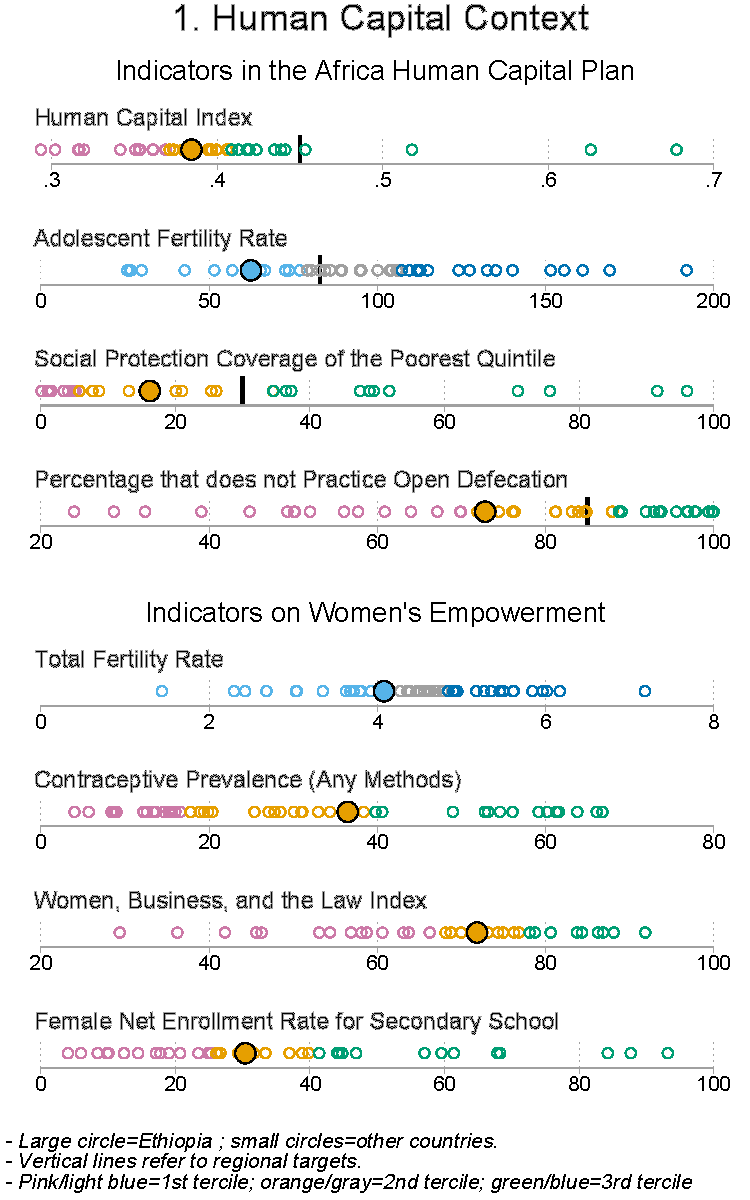
\includegraphics[width=1\linewidth]{charts/all_mf_ETH} \end{flushright}
\vspace{3mm}

\begin{flushright}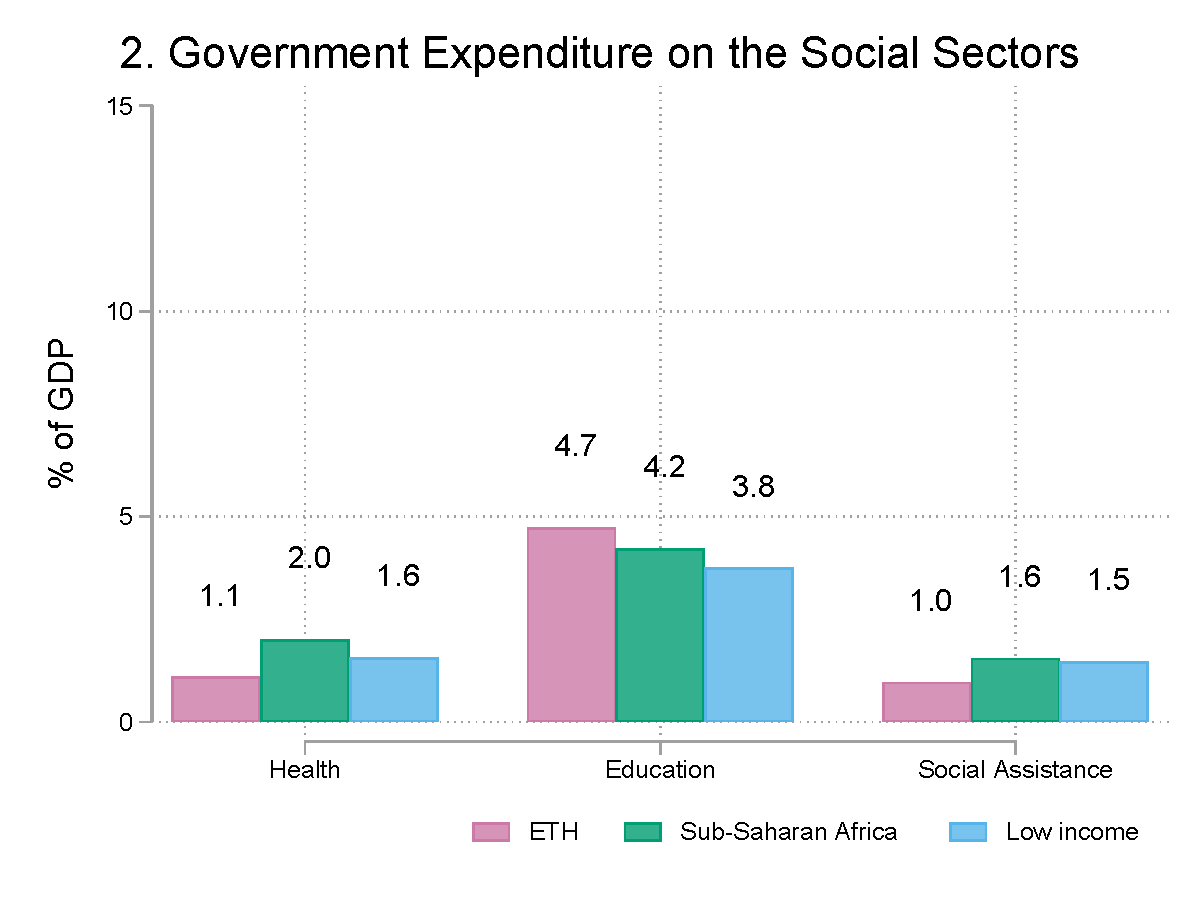
\includegraphics[width=1\linewidth,height=1.2\textheight]{charts/socsec_ETH} \end{flushright}
\vspace{3mm}

\begin{itemize}
\tightlist
\item
  \textbf{Efficiency of Spending.} The HCI in Ethiopia is \textbf{lower}
  than what would be predicted for its level of per capita spending on
  the social sectors.
\end{itemize}

\begin{center}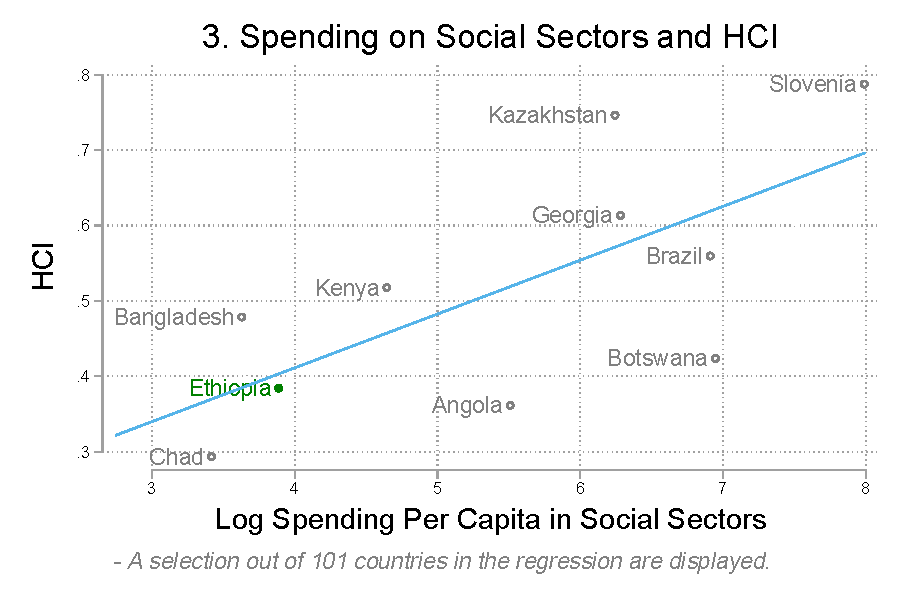
\includegraphics[width=1\linewidth,height=0.5\textheight]{charts/efficiency_ETH} \end{center}

\begin{itemize}
\tightlist
\item
  \textbf{Domestic Resource Mobilization.} The tax revenue in Ethiopia
  is \textbf{7.7} percent of GDP. This is lower than both the regional
  average (16.1) and the average for its income group (14.3).
\end{itemize}

\begin{flushright}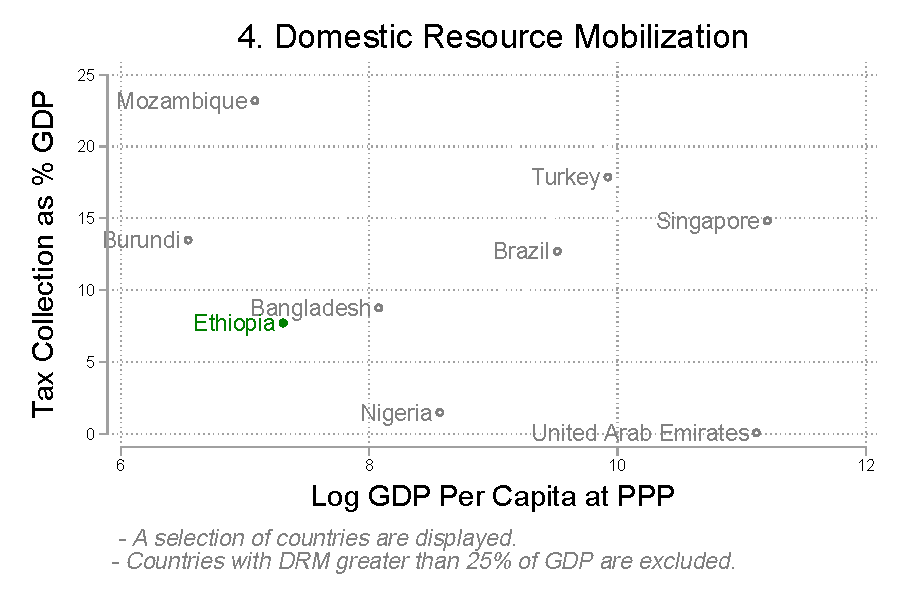
\includegraphics[width=1\linewidth,height=0.5\textheight]{charts/drm_ETH} \end{flushright}

\begin{itemize}
\item
  \textbf{Building Human Capital.} The Country Policy and Institutional
  Assesment rating for building human resources in Ethiopia is
  \textbf{4.5} (1 is low and 6 is high). This is higher than both the
  regional average (3.5) and the average for its income group (3.5).
  This indicator assesses the national policies and public and private
  sector service delivery that affect access to and quality of health
  and education services.
\item
  \textbf{Identification} In Ethiopia, \textbf{64.5 percent} of the
  population does not have proof of identity. This is higher than both
  the regional average (33.8) and the average for its income group
  (34.6).
\item
  \textbf{Statistical Data on Human Capital} In Ethiopia, the latest
  available data on stunting rates is from 2016. Similarly, the last
  available data point on Harmonized Learning Outcomes is from 2010.
\end{itemize}

\hypertarget{section-3}{%
\subsubsection{\texorpdfstring{\textcolor{bondiblue}{\textbf{H\small{OW IS THE WORLD BANK SUPPORTING THE EFFORT?}}}}{}}\label{section-3}}

The following table summarizes the World Bank investments in Human
Development for Ethiopia, including measures of volume, performance, and
other relevant indicators.

\definecolor{asparagus}{RGB}{3, 158, 115}
\definecolor{blush}{RGB}{204 121 167}
\definecolor{arylideyellow}{RGB}{230 159 0}
\definecolor{blue(ncs)}{rgb}{0.0, 0.53, 0.74}
\definecolor{ashgrey}{rgb}{0.7, 0.75, 0.71}
\definecolor{bleudefrance}{rgb}{0.19, 0.55, 0.91}
\definecolor{iceberg}{rgb}{0.44, 0.65, 0.82}
\begin{table}[H]
\small
\begin{tabular}{lcccc}
\textbf{World Bank Investments in HD}       & \textbf{}        & \textbf{}      & \textbf{} & \textbf{} \\\hline
\textbf{Indicator}       & \textbf{HD}        & \textbf{Edu}      & \textbf{HNP} & \textbf{SPJ} \\\hline
\cellcolor{iceberg}HD Portfolio      &    \cellcolor{iceberg}     &   \cellcolor{iceberg}    & \cellcolor{iceberg} & \cellcolor{iceberg} \\ \hline
USD (million)                    &      3,558                &     300                &   250        & 3,008         \\
Percentage of total        &        \cellcolor{asparagus}32               &     \cellcolor{arylideyellow}      3           &     \cellcolor{arylideyellow}  2         & \cellcolor{asparagus}27 \\
Diff. with perc. for regional average &         +9              &  -3                 &  -6        & +18 \\
Diff. with perc. for income group avg   &       +4                &     -3                  &    -9          &  +18 \\  \hline
\cellcolor{iceberg}HD FY 20 Lending Program      &   \cellcolor{iceberg}      & \cellcolor{iceberg}      & \cellcolor{iceberg} & \cellcolor{iceberg} \\ \hline
USD (million)                    &      560                &    60                 &    0      &  500     \\
Percentage of total        &      \cellcolor{asparagus}  100               &       \cellcolor{asparagus} 10            &    \cellcolor{blush} 0             &  \cellcolor{asparagus}89.3  \\
Diff. with perc. for regional average &   +44           &   -20           &       -9   &   +77   \\
Diff. with perc. for income group avg   &     +64                   &  +2                &     -11        &   +73   \\  \hline
\cellcolor{iceberg}HD Performance      &   \cellcolor{iceberg}      & \cellcolor{iceberg}      & \cellcolor{iceberg} & \cellcolor{iceberg} \\ \hline
Average Development Outcome (DO)                  &     \cellcolor{arylideyellow} 3.3               &   \cellcolor{blush} 3                 &     \cellcolor{blush}3     &  \cellcolor{arylideyellow}3.5     \\
Difference with DO for region   &    -0.2     &        -0.3               &      -0.57           &  -0.15 \\
Difference with DO for income group   &      -0.11                &      -0.34               &      -0.57          &   -0.06  \\
Perc. Satisfactory DO                 &     100               &    100                 &     \ 100     &  100     \\
Average Implementation Progress (IP)         &      \cellcolor{blush} 3               &   \cellcolor{blush}    3               &   \cellcolor{blush} 3             & \cellcolor{blush}3  \\
Difference with IP for region   &      -0.32          &       -0.22               &       -0.34          &    0.51 \\
Difference with IP for income group   &      -0.30                &       -0.23               &      -0.40             &   -0.36  \\
Perc. Satisfactory IP                 &      100               &    100                 &     \ 100     &  100     \\
Disbursement ratio (DR) &        \cellcolor{asparagus}54.5              &        .            &  .               & \cellcolor{asparagus}54.5 \\
Difference with DR for region   &    15.5               &     .         &    .           &  +2 \\
Difference with DR for income group   &     +10                &     .              &     .           &   -5  \\\hline
\cellcolor{iceberg}Other indicators      &   \cellcolor{iceberg}      & \cellcolor{iceberg}      & \cellcolor{iceberg} & \cellcolor{iceberg} \\ \hline
Average project size (PS) (USD mill.)                 &    \cellcolor{asparagus}  351                &    \cellcolor{asparagus}  300                 &    \cellcolor{asparagus}  250     &  \cellcolor{asparagus}   752       \\
Difference with PS for region        &     +255               &         +293               &   190                &   +664 \\
Difference with PS for income group   &    +277              &        +242            &  178             & +659 \\
Perc. of portfolio that is co-TTL'd (CTT)    &      \cellcolor{asparagus}  62                &    \cellcolor{blush}     0               &    \cellcolor{blush}    0           &   \cellcolor{asparagus} 73  \\
Diff. with CTT for region (perc. points)  &     +36                &      -15               &        -31          &    +42\\
Diff. with CTT income group (perc. points)  &     +32                &     -21               &       -35           &  +37\\
\hline
                         \multicolumn{5}{l}{Note: a) Pink indicates that the value is within the first tercile of the} \\
                         \multicolumn{5}{l}{distribution for all the countries. Orange indicates that the value is } \\
                         \multicolumn{5}{l}{is within the second tercile. Green indicates that it is within the third} \\
                         \multicolumn{5}{l}{tercile. b) FY20 lending program includes only projects rated A, B and } \\
                          \multicolumn{5}{l}{unrated. c) DO and IP are on a scale of 1 to 5 where 1 is Unsatisfactory } \\
                          \multicolumn{5}{l}{and5 is Highly Satisfactory. d) Data as of July 15, 2019.} \\
\end{tabular}
\end{table}

\begin{itemize}
\item
  \textbf{Human Capital Policy Operations.} Currently, the pipeline for
  Ethiopia \textbf{does not} include any Development Policy Operations
  with a Human Capital-related component or prior action.
\item
  \textbf{Women Empowerment Project.} Currently, Ethiopia \textbf{does
  not} have an active project focused on women empowerment or on sexual
  and reproductive health.
\end{itemize}

\noindent

\rule{9cm}{0.4pt}

The present scorecard aims to be a conversation starter on some of the
main indicators that show progress towards human capital outcomes. The
list of indicators presented here is not exhaustive and should be
complemented with more specific variables. ~

The sources for the different indicators come from the Human Capital
Project, the World Development Indicators, and the World Bank's internal
system to monitor investments. ~

For more information, please contact the Africa Human Capital team:
\href{mailto:AFR_HCP_Team@worldbankgroup.org}{\nolinkurl{AFR\_HCP\_Team@worldbankgroup.org}}


\end{document}
